\boxde
\BTTN
\Opensolutionfile{ans}[ans/2D1-3-DEON-2]
\begin{ex}%[Dự án tex hóa đề cương Mariecurie - Biên soạn Thầy Nguyễn Ngọc Nguyên]%[2D1B3-2]
    Hàm số $y=f(x)$ liên tục và có bảng biến thiên trên đoạn $[-1;3]$ như hình bên.
    \begin{center}
        
\begin{tikzpicture}
            \tkzTabInit[espcl=3]
            {$x$ /.6, $y'$ /.6,$y$ /1.8}
            {$-1$,$0$,$2$,$3$}
            \tkzTabLine{,+,d ,-,$0$,+}
            \tkzTabVar{ -/$0$,+/$5$,-/$1$,+/$4$}
        \end{tikzpicture}
    \end{center}
    Giá trị lớn nhất của hàm số trên đoạn $[-1;3]$ bằng
    \choice
    {$f(-1)$}
    {$f(3)$}
    { \True $f(0)$}
    { $f(2)$}
    \loigiai
    {
        Dựa vào bảng biến thiên ta thấy hàm số đạt giá trị lớn nhất tại $x=0$.
    }
\end{ex}
\begin{ex}%[Dự án tex hóa đề cương Mariecurie - Biên soạn Thầy Nguyễn Ngọc Nguyên]%[2D1B3-2]
    Hàm số $y=f(x)$ liên tục trên $\mathbb{R}$ và có bảng biến thiên như hình bên.
    \begin{center}
        
\begin{tikzpicture}
            \tkzTabInit[espcl=3]
            {$x$ /.6, $y'$ /.6,$y$ /1.8}
            {$-\infty$,$0$,$1$,$+\infty$}
            \tkzTabLine{,-,$0$, +,d ,-,}
            \tkzTabVar{ +/$+\infty$,-/$1$,+/$5$,-/$2$}
        \end{tikzpicture}
    \end{center}
    Mệnh đề nào dưới đây\textbf{ sai}?
    \choice
    {$y_\text{cđ}=5$}
    {\True $\max\limits_{\mathbb{R}}y=5$}
    {$y_\text{ct}=0$}
    {$\min\limits_{\mathbb{R}}y=1$}
    \loigiai
    {
        Vì $\lim \limits_{x \to -\infty} f(x)=+\infty$ nên hàm số không tồn tại giá trị lớn nhất trên tập $\mathbb{R}$. Vậy mệnh đề $\max\limits_{\mathbb{R}}y=5$ là sai.
    }
\end{ex}
\begin{ex}%[THPTQG 2020 câu 35 đề 103]%[2D1B3-1]
    Giá trị nhỏ nhất của hàm số $f(x)=x^3-30x$ trên đoạn $[2;19]$ bằng
    \choice
    {$20\sqrt{10}$}
    {$-63$}
    {\True $-20\sqrt{10}$}
    {$-52$}
    \loigiai{
        Ta có $f’(x)=3x^2-30$; $f'(x)=0\Leftrightarrow \hoac{&x=\sqrt{10}\\&x=-\sqrt{10}.}$\\
        Do xét trên đoạn $[2;19]$ nên ta nhận $x=\sqrt{10}$.\\
        Khi đó $f(2)=-52$, $f(19)=6289$, $f\left(\sqrt{10}\right)=-20\sqrt{10}\approx -63{,}25$.\\
        Vậy giá trị nhỏ nhất của $f(x)$ trên đoạn $[2;19]$ là $f\left(\sqrt{10}\right)=-20\sqrt{10}$.
    }
\end{ex}
\begin{ex}%[THPTQG 2020 câu 29 đề 104]%[2D1B3-1]
    Giá trị nhỏ nhất của hàm số $f(x)=x^3-33x$ trên đoạn $[2;19]$ bằng
    \choice
    {$-72$}
    {\True $-22\sqrt{11}$}
    {$-58$}
    {$22\sqrt{11}$}
    \loigiai{
        Hàm số $f(x)$ liên tục trên đoạn $[2;19]$, có $f'(x)=3x^2-33$, $f'(x)=0\Leftrightarrow \hoac{&x=-\sqrt{11}\notin (2;19)\\&x=\sqrt{11}\in (2;19).}$\\
        Lại có $f(2)= -58$, $f\left(\sqrt{11}\right)= -22\sqrt{11}$, $f(19)= 6232$. Vậy $\min\limits_{[2;19]}f(x)= -22\sqrt{11}$.
    }
\end{ex}
\begin{ex}%[Dự án tex hóa đề cương Mariecurie - Biên soạn Thầy Nguyễn Ngọc Nguyên]%[2D1Y3-1]
    Giá trị lớn nhất của hàm số $f(x)=x^4-4x^2+5$ trên đoạn $[-2;3]$ bằng
    \choice
    {\True $50$}
    {$5$}
    {$1$}
    {$122$}
    \loigiai{
        Ta có $y'=4x^3-8x$. Giải $y'=0 \Leftrightarrow \hoac{&x=0 \in [-2;3] \\ &x=\sqrt{2} \in [-2;3] \\ &x=-\sqrt{2} \in [-2;3].}$\\
        Tính $f(-\sqrt{2})=1$, $f(0)=5$, $f(\sqrt{2})=1$, $f(3)=50$. \\
        Vậy	$\max \limits_{[-2;3]} f(x)=50$.
    }
\end{ex}
\begin{ex}%[Dự án tex hóa đề cương Mariecurie - Biên soạn Thầy Nguyễn Ngọc Nguyên]%[2D1Y3-1]
    Giá trị nhỏ nhất của hàm số $y=x^4-x^2+13$ trên đoạn $[-2;3]$ bằng
    \choice
    {$\dfrac{49}{4}$}
    {\True $\dfrac{51}{4}$}
    {$13$}
    {$\dfrac{51}{2}$}
    \loigiai{
        Ta có $y'=4x^3-2x$. Giải $y'=0 \Leftrightarrow \hoac{&x=0 \in [-2;3] \\ &x=\dfrac{\sqrt{2}}{2} \in [-2;3] \\ &x=-\dfrac{\sqrt{2}}{2} \in [-2;3].}$\\
        Tính $f(-2)=25$, $f \left(-\dfrac{\sqrt{2}}{2}\right )=\dfrac{51}{4}$, $f \left( \dfrac{\sqrt{2}}{2} \right )=\dfrac{51}{4}$, $f(3)=85$.	\\
        Vậy $\min \limits_{[-2;3]} f(x)= \dfrac{51}{4}$.
    }
\end{ex}
\begin{ex}%[Nguyễn Trần Phong, Dự án 6 đề cương HKI k12 Marie]%[2D1B3-1]
    Giá trị nhỏ nhất của hàm số $y=\dfrac{2x-1}{x+1}$ trên đoạn $[1;3]$ bằng
    \choice
    {$ \dfrac{5}{4}$}
    {$ 2$}
    {\True $ \dfrac{1}{2}$}
    {$\dfrac{7}{2} $}
    \loigiai{
        Ta có $y'= \dfrac{3}{(x+1)^2} >0$ với mọi $x \in [1;3]$.\\
        Suy ra hàm số đồng biến trên $[1;3]$.\\
        Vậy $\displaystyle \min_{[1;3]} y = y(1)= \dfrac{1}{2}$.}
\end{ex}
\begin{ex}%[Nguyễn Trần Phong, Dự án 6 đề cương HKI k12 Marie]%[2D1B3-1]
    Cho hàm số $y= \dfrac{3x-1}{x-3}$. Gọi $M$, $m$ lần lượt là giá trị lớn nhất, giá trị nhỏ nhất của hàm số trên đoạn $[0;2]$. Giá trị của $M+m$ bằng
    \choice
    {$4 $}
    {\True $- \dfrac{14}{3} $}
    {$ \dfrac{14}{3}$}
    {$\dfrac{3}{5} $}
    \loigiai{
        Ta có $y' = \dfrac{-8}{(x-3)^2}<0$ với mọi $x \in [0;2]$.\\
        Suy ra hàm số nghịch biến trên đoạn $[0;2]$.\\
        Do đó $m = \displaystyle \min_{[0;2]}y = y(2)= -5$; $M = \displaystyle \max_{[0;2]} y = y(0) = \dfrac{1}{3}$.\\
        Vậy $M+ m = - \dfrac{14}{3}$.}
\end{ex}
\begin{ex}%[Dự án tex hóa đề cương Mariecurie - Biên soạn Thầy Nguyễn Ngọc Nguyên]%[2D1B3-1]
    \immini{	Cho hàm số $f(x)$ liên tục trên đoạn $[-1;5]$ và có đồ thị như hình vẽ bên. Gọi $M,m$ lần lượt là giá trị lớn nhất, nhỏ nhất của hàm số trên đoạn $[-1;5]$. Giá trị $M+m$ bằng }
    {
        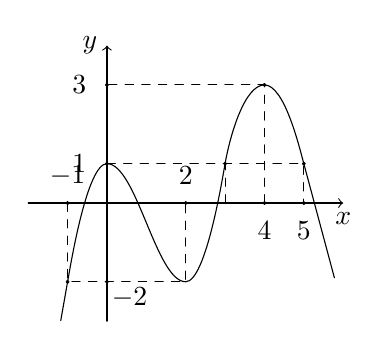
\begin{tikzpicture}[line cap=round, line join=round, scale=0.5]
            \draw[->](-2,0)--(6,0)node[below]{$x$};
            \draw[->](0,-3)--(0,4)node[left]{$y$};
            \draw([shift={(-100:1)}]-1,-2)--(-1,-2)..controls++(80:0.5) and++(180:0.5)..(0,1)..controls++(0:0.75) and ++(180:0.75)..(2,-2)..controls++(0:0.5) and ++(-100:0.5)..(3,1)..controls ++(80:0.75) and ++(180:0.5)..(4,3)..controls++(0:0.5) and++(105:0.5)..(5,1)--++(-75:3);
            \draw[dashed](-1,0)--(-1,-2)--(2,-2)--(2,0)(0,1)--(5,1)--(5,0)(3,0)--(3,1)(4,0)--(4,3)--(0,3);
            \foreach \x/\y/\m/\g in{-1/-2//0,0/-2/-2/-35,3/1//0,4/0/4/-90,5/0/5/-90,5/1//0,0/1/1/180,-1/0/-1/90,2/0/2/90,0/3/3/180,4/3//0}
            \draw[fill=black](\x,\y)circle(1pt)node[shift={(\g:0.35)}]{$\m$};
        \end{tikzpicture}
    }
    \choice
    {$4$}
    {$5$}
    {$6$}
    {\True $1$}
    \loigiai{ Dựa vào đồ thị ta có $M=3$ và $m=-2$. Do đó $M-m=3+(-2)=1$.
    }
\end{ex}
\begin{ex}%[Dự án tex hóa đề cương Mariecurie - Biên soạn Thầy Nguyễn Ngọc Nguyên]%[2D1B3-1]
    \immini{	Cho hàm số $f(x)$ liên tục trên đoạn $[-2;3]$ và có đồ thị như hình bên. Gọi $M,m$ lần lượt là giá trị lớn nhất, nhỏ nhất của hàm số đã cho trên đoạn $[-2;3
        ]$. Giá trị của $M+m$ bằng}
    {
        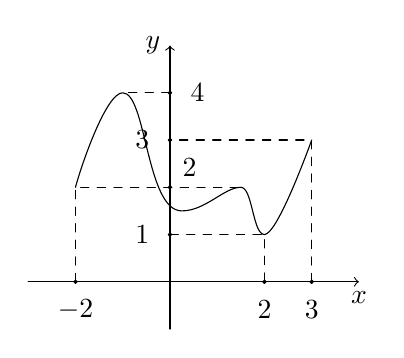
\begin{tikzpicture}[line cap=round, line join=round, scale=0.6]
            \draw[->](-3,0)--(4,0)node[below]{$x$};
            \draw[->](0,-1)--(0,5)node[left]{$y$};
            \draw(-2,2)..controls++(75:0.5) and++(180:0.35)..(-1,4)..controls++(0:0.5) and ++(180:0.75)..(0.25,1.5)..controls++(0:0.5) and ++(180:0.35)..(1.5,2)..controls ++(0:0.25) and ++(180:0.25)..(2,1)..controls++(0:0.25) and ++(-110:0.5)..(3,3);
            \draw[dashed](-2,0)--(-2,2)--(1.5,2)(0,1)--(2,1)--(2,0)(3,0)--(3,3)--(0,3)(0,4)--(-1,4);
            \foreach \x/\y/\m/\g in{-2/0/-2/-90,0/2/2/45,0/1/1/180,2/0/2/-90,3/0/3/-90,0/3/3/180,0/4/4/0}
            \draw[fill=black](\x,\y)circle(1pt)node[shift={(\g:0.35)}]{$\m$};
        \end{tikzpicture}
    }
    \choice
    {$2$}
    {$1$}
    {$4$}
    {\True $5$}
    \loigiai
    {
        Ta có $M=4$ và $m=1$, do đó $M+m=5$.
    }
\end{ex}
\begin{ex}%[Nguyễn Trần Phong, Dự án 6 đề cương HKI k12 Marie]%[2D1B3-1]
    Giá trị nhỏ nhất của hàm số $f(x)= \sin^5 x - 2 \sin^3 x +1$ bằng
    \choice
    {$ -2$}
    {$ -1$}
    {$ 1$}
    {\True $0 $}
    \loigiai{
        Đặt $t= \sin x$, $t \in [-1;1]$. Khi đó ta được $g(t)= t^5 -2t^3 +1$ với $t \in [-1;1]$.\\
        Suy ra $g'(t) = 5t^4 -6t^2.$\\
        Cho $g'(t) =0 \Leftrightarrow \hoac{& t=0 \in [-1;1]\\& t= \pm \dfrac{\sqrt{3}}{5} \notin [-1;1].}$\\
        Xét $g(-1)=2$; $g(0) =1$; $g(1)= 0$.\\
        Vậy $ \displaystyle \min_{\mathbb{R}}f(x) = \displaystyle \min_{[-1;1]} g(t)= 0$.}
\end{ex}
\begin{ex}%[Nguyễn Trần Phong, Dự án 6 đề cương HKI k12 Marie]%[2D1B3-3]
    Tổng giá trị lớn nhất và giá trị nhỏ nhất của hàm số $f(x) = \sin^4 x + \cos^4 x $ bằng
    \choice
    {\True $\dfrac{3}{2} $}
    {$\dfrac{1}{2} $}
    {$- \dfrac{1}{2} $}
    {$- \dfrac{3}{2} $}
    \loigiai{
        Ta có $f(x)= \sin^4 x + \cos^4 x = 1 - \dfrac{1}{2} \sin^2 2x$.\\
        Suy ra $f(x) \in \left[\dfrac{1}{2} ;1 \right]$.\\
        Vậy tổng giá trị lớn nhất và nhỏ nhất của hàm số là $\dfrac{1}{2} + 1 = \dfrac{3}{2}.$}
\end{ex}
\begin{ex}%[Nguyễn Trần Phong, Dự án 6 đề cương HKI k12 Marie]%[2D1K3-1]
    Với giá trị nào của $m$ thì hàm số $f(x)= - \dfrac{1}{3} x^3 -x + m +1$ đạt giá trị lớn nhất bằng $5$ trên $[0;3]$?
    \choice
    {$m= \dfrac{8}{3}$}
    {$ m= \dfrac{16}{3} $}
    {$ 16$}
    {\True $ 4$}
    \loigiai{
        Ta có $f'(x)= -x^2 -1<0$ với mọi $x \in [0;3]$.\\
        Suy ra hàm số nghịch biến trên đoạn $[0;3]$ và do đó $\displaystyle \max_{[0;3]} f(x) = f(0) = m+1$.\\
        Theo giả thiết, $m+1 = 5 \Leftrightarrow m = 4.$}
\end{ex}
\begin{ex}%[2D1K3-1]%[Dự án TEX hóa đề cương Marie Curie - Ân Trương]
    Cho hàm số $ f(x)=\dfrac{mx-1}{x+m} $ ($ m $ là tham số thực) thỏa mãn $ \max\limits_{[0 ; 1]} f(x)=2 $. Khi đó giá trị $ m $ bằng
    \choice
    {$m=\dfrac{1}{2}$}
    {$m=-\dfrac{1}{2}$}
    {\True$m=-3$}
    {$m=1$}
    \loigiai{
        Tập xác định $ \mathscr{D} = \mathbb{R} \setminus\{-m\}$.\\
        Để hàm số có giá trị lớn nhất trên $ [0;1] $ thì $ m\notin [0;1] $.\\
        Ta có $ f'(x)=\dfrac{m^2+1}{(x+m)^{2}} >0, \forall x \ne -m$.\\
        $ \Rightarrow \max\limits_{[0;1]}f(x)=f(1)=\dfrac{m-1}{1+m} $.\\
        Theo đề bài
        \begin{eqnarray*}
            &&\max\limits_{[0;1]}f(x)=2\\
            &\Leftrightarrow& \dfrac{m-1}{1+m}=2\\
            &\Leftrightarrow& m-1=2m+2\\
            &\Leftrightarrow& m=-3.
        \end{eqnarray*}
    }
\end{ex}
\begin{ex}%[Dự án DeKiemtradinhki-Lan 1]%[Soạn: Ngụy Như Thái-Phản biện:Anh Phan]%[2D1K3-6]%
    Một vật chuyển động theo quy luật $s=-\dfrac{1}{3}t^3+6t^2$ với $t$ (giây) là khoảng thời gian tính từ khi vật bắt đầu chuyển động và $s$ (mét) là quãng đường vật di chuyển được trong khoảng thời gian đó. Hỏi trong khoảng thời gian $9$ giây kể từ khi bắt đầu chuyển động, vận tốc lớn nhất của vật là bao nhiêu?
    \choice
    {$243$ m/s}
    {\True $36$ m/s}
    {$144$ m/s}
    {$27$ m/s}
    \loigiai{
        Vận tốc của vật tính bởi công thức $v=s'=-t^2+12t=-(t-6)^2+36$.\\
        Suy ra vận tốc của vật lớn nhất bằng $36$ m/s khi $t=6$ (giây).}
\end{ex}
\begin{ex}%[2D1K3-1]%[Dự án TEX hóa đề cương Marie Curie - Ân Trương]
    \immini
    {
        Cho hàm số $ y=f(x) $ có đạo hàm liên tục trên $ \mathbb{R} $ và đồ thị hàm số $ y=f'(x) $ như hình vẽ. Đặt $ g(x)=2f(x)-(x+1)^2 $. Biết $ f(-2)=f(3) $. Mệnh đề nào dưới đây đúng ?
        \choice
        {$\max\limits_{[-2; 3]}g(x)=g(3),\quad \min\limits_{[-2; 3]}g(x)=g(-2)$}
        {\True$\max\limits_{[-2; 3]}g(x)=g(2),\quad \min\limits_{[-2; 3]}g(x)=g(3)$}
        {$\max\limits_{[-2; 3]}g(x)=g(2),\quad \min\limits_{[-2; 3]}g(x)=g(-2)$}
        {$\max\limits_{[-2; 3]}g(x)=g(-2),\quad \min\limits_{[-2; 3]}g(x)=g(2)$}
    }
    {
        \begin{tikzpicture}[>=stealth,x=1cm,y=1cm,scale=0.8,font=\footnotesize]
            \path
            (-2,0) coordinate (Af)(2.5,0) coordinate (Bf)(0,4) coordinate (Df)(0,-3) coordinate (Cf)
            (0,0) coordinate (O)node[above right]{$ O $}
            (-1.2,-0.7) coordinate (P)
            (-0.4,1.8) coordinate (N)node[shift={(-0.8,0.2)}]{$ y=f'(x)$}
            (0.4,1.5) coordinate (M1)
            (1,2.5) coordinate (M2)
            (1.7,1.5) coordinate (M3)
            (2.2,3.3) coordinate (M4)
            (-1.3,-1.2) coordinate (P1)
            (2.25,3.7) coordinate (M6)
            ;
            %	\draw[red] (P)--(N)--(M1)--(M2)--(M3)--(M4);
            \draw[name path=ox] (Af)--(Bf);
            \draw[name path=oy] (O)--(Df);
            \draw[name path=fx,thick,black]
            (P1)--(P)..controls +(70:0.25) and+(-160:0.5)..(N)
            ..controls +(10:0.25) and+(175:0.25)..(M1)
            ..controls +(-5:0.25) and+(-175:0.25)..(M2)
            ..controls +(5:0.25) and+(170:0.25)..(M3)
            ..controls +(-5:0.25) and+(-100:0.25)..(M4)--(M6)
            ;
            \path[name path=d](P)--(M4);
            \path[name intersections={of=fx and d, by={P,M5,M4}}] ;
            \path[name intersections={of=fx and ox, by={A}}] ;
            %	Vẽ hệ trục tọa dộ:
            \draw[->] (-1.5,0)--(0,0)--(3,0) node[below]{$x$};
            \draw[->] (0,-1.5) --(0,4) node[left]{$y$};
            %	Node các điểm
            \foreach \p in {P,M5,M4,A,O}
            \fill (\p) circle (1.5pt) ;
            %	Vẽ nét đứt+node:
            \foreach \p/\n/\r in {P/-2/150,M5/2/-90,M4/3/-90}
            \draw[dashed](\p)--($(Af)!(\p)!(Bf)$)node[shift={(\r:3mm)}]{$ \n $} ;
            \foreach \p/\n/\r in {P/-1/0,M5/3/180,M4/4/180}
            \draw[dashed](\p)--($(Cf)!(\p)!(Df)$)node[shift={(\r:2mm)}]{$ \n $} ;
        \end{tikzpicture}
    }
    \loigiai{
        Ta có $ g'(x)=2\cdot f'(x)-2(x+1) $.\\
        Cho
        \begin{eqnarray*}
            &&g'(x)=0 \\
            &\Leftrightarrow&2\cdot f'(x)-2(x+1)=0\\
            &\Leftrightarrow&f'(x)=x+1.
        \end{eqnarray*}
        \immini
        {
            Đây là phương trình hoành độ giao điểm của đồ thị hàm số $ y=f'(x) $ và PTĐT $ y=x+1 $.\\
            Dựa vào đồ thị, ta lập được bảng biến thiên của hàm số $ y=g(x) $
            \begin{center}
                
\begin{tikzpicture}
                    \tkzTabInit[nocadre=false,lgt=1.2,espcl=2.5,deltacl=0.7]
                    {$x$ /0.6,$g’(x)$ /0.6,$g(x)$ /2}
                    {$-2$,$2$,$3$}
                    \tkzTabLine{,+,0,-,}
                    \tkzTabVar{-/$g(-2)$,+/$g(2)$,-/$g(3)$}
                \end{tikzpicture}
            \end{center}
        }
        {
            \begin{tikzpicture}[>=stealth,x=1cm,y=1cm,scale=1,font=\footnotesize]
                \path
                (-2,0) coordinate (Af)(2.5,0) coordinate (Bf)(0,4) coordinate (Df)(0,-3) coordinate (Cf)
                (0,0) coordinate (O)node[above right]{$ O $}
                (-1.2,-0.7) coordinate (P)
                (-0.4,1.8) coordinate (N)node[shift={(-0.8,0.2)}]{$ y=f'(x)$}
                (0.4,1.5) coordinate (M1)
                (1,2.5) coordinate (M2)
                (1.7,1.5) coordinate (M3)
                (2.2,3.3) coordinate (M4)
                (-1.3,-1.2) coordinate (P1)
                (2.25,3.7) coordinate (M6)
                ;
                %	\draw[red] (P)--(N)--(M1)--(M2)--(M3)--(M4);
                \draw[name path=ox] (Af)--(Bf);
                \draw[name path=oy] (O)--(Df);
                \draw[name path=fx,thick,black]
                (P1)--(P)..controls +(70:0.25) and+(-160:0.5)..(N)
                ..controls +(10:0.25) and+(175:0.25)..(M1)
                ..controls +(-5:0.25) and+(-175:0.25)..(M2)
                ..controls +(5:0.25) and+(170:0.25)..(M3)
                ..controls +(-5:0.25) and+(-100:0.25)..(M4)--(M6)
                ;
                \draw[shorten >=-0.5cm, shorten <=-0.5cm,name path=d,black](P)--(M4);
                \path[name intersections={of=fx and d, by={P,M5,M4}}] ;
                \path[name intersections={of=fx and ox, by={A}}] ;
                %	Vẽ hệ trục tọa dộ:
                \draw[->] (-1.3,0)--(0,0)--(3,0) node[below]{$x$};
                \draw[->] (0,-1.5) --(0,4) node[left]{$y$};
                %	Node các điểm
                \foreach \p in {P,M5,M4,A,O}
                \fill (\p) circle (1.5pt) ;
                %	Vẽ nét đứt+node:
                \foreach \p/\n/\r in {P/-2/150,M5/2/-90,M4/3/-90}
                \draw[dashed](\p)--($(Af)!(\p)!(Bf)$)node[shift={(\r:3mm)}]{$ \n $} ;
                \foreach \p/\n/\r in {P/-1/0,M5/3/180,M4/4/180}
                \draw[dashed](\p)--($(Cf)!(\p)!(Df)$)node[shift={(\r:2mm)}]{$ \n $} ;
            \end{tikzpicture}
        }
        Ta có
        \begin{eqnarray*}
            g(-2)&=&2\cdot f(-2)-(-2+1)^2=2\cdot f(-2)-1\\
            g(3)&=&2\cdot f(3)-(3+1)^2=2\cdot f(3)-16\\
            &\xrightarrow{f(3)=f(-2)}&g(3)<g(-2).
        \end{eqnarray*}
        Vậy $\max\limits_{[-2; 3]}g(x)=g(2),\quad \min\limits_{[-2; 3]}g(x)=g(3)$.
    }
\end{ex}
\begin{ex}
    \immini
    {
        cho hàm số, $y=f(x)$ liên tục trên $\mathbb{R}$, có đồ thị như hình vẽ. Tìm tham số $m$ để bất phương trình $f(x)\geq m$ có nghiệm $x\in [-1;2]$.
        \choice
        {\True $m\leq 5$}
        {$m\geq 5$}
        {$m\leq -1$}
        {$m\geq -1$}
    }
    {
        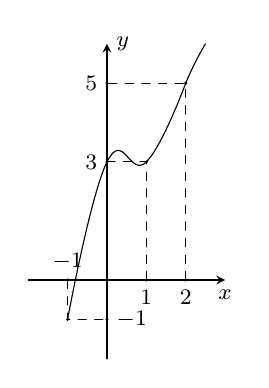
\begin{tikzpicture}[>=stealth,line join=round,line cap=round,font=\footnotesize,scale=.5]
            \draw[->] (0,-2)--(0,6)node[right]{$y$};
            \draw[->] (-2,0)--(3,0)node[below]{$x$};
            \draw plot[smooth,tension=.75] coordinates{(-1,-1) (0,3) (1,3) (2,5)};
            \draw (2,5)to[out=67,in=-120](2.5,6);
            \draw[dashed](-1,0)node[above]{$-1$}--(-1,-1)--(0,-1)node[right]{$-1$}
            (1,0)node[below]{$1$}--(1,3)--(0,3)node[left]{$3$}
            (2,0)node[below]{$2$}--(2,5)--(0,5)node[left]{$5$};
            \foreach \d in{(-1,0),(1,0),(2,0),(0,-1),(0,3),(0,5),(-1,-1),(1,3),(2,5),(0,0)}\fill \d circle (1.2pt);
        \end{tikzpicture}
    }
\end{ex}
%%==========Câu 7
\begin{ex}%[Phạm Đình Quang-DA1]%[2D1K1-4]
    \immini
    {
        Cho hàm số $y=f(x)$ liên tục trên đoạn $[-2;6]$, có đồ thị như hình vẽ. Tìm tất cả các tham số $m$ để bất phương trình $f(\sin x)\geq m$ có nghiệm.
        \choice
        {\True $m\leq 5$}
        {$m\geq 1$}
        {$m\leq -4$}
        {$m\geq 1$}
    }
    {
        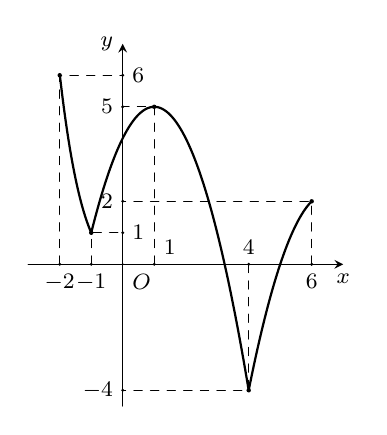
\begin{tikzpicture}[scale=.4,>=stealth, font=\footnotesize, line join=round, line cap=round]
            % đồ thị 1: y=f(x)=a1*x^4 + b1*x^2
            \def\af{0.17} \def\bf{0.83}
            % đồ thị 2: y=g(x)= a2*x^2 + b2*x +c2
            \def\ag{-1} \def\bg{2} \def\cg{4}
            % đồ thị 3: y=h(x)=a3*x^2 + b3*x +c3
            \def\ah{-1} \def\bh{13} \def\ch{-40}
            \def\xmin{-3} \def\xmax{7}
            \def\ymin{-4.5} \def\ymax{7}
            %\draw[help lines] (-5,-5) grid (5,5);
            \draw[->] (\xmin,0)--(\xmax,0) node [below]{$x$};
            \draw[->] (0,\ymin)--(0,\ymax) node [left]{$y$};
            \fill[name=O] (0,0) circle (1pt) node[below right] {$O$};
            \clip (\xmin+0.1,\ymin+0.1) rectangle (\xmax-0.5,\ymax-0.1);
            \draw[thick,smooth,samples=300,domain= -2:-1 ] plot(\x,{\af*(\x)^4+\bf*(\x)^2});
            \draw[thick,smooth,,samples=300,domain=-1:4] plot(\x,{\ag*(\x)^2+\bg*(\x)+\cg});
            \draw[thick,smooth, samples=300,domain=4:6] plot(\x,{\ah*(\x)^2+\bh*(\x)+\ch});
            \draw[dashed] (-2,0)|-(0,6)
            (-1,0)|-(0,1)
            (1,0)|-(0,5)
            (4,0)|-(0,-4)
            (6,0)|-(0,2);
            \foreach \x/\p in {-2/-92,-1/-93,1/45,4/90,6/-90}
            \fill (\x,0) circle (1.5pt)coordinate[label=\p:$\x$];
            \foreach \y/\p in {-4/180,1/0,2/180,5/180,6/0}
            \fill (0,\y) circle (1.5pt)coordinate[label=\p:$\y$];
            \foreach \p in {(-2,6),(-1,1),(1,5),(4,-4),(6,2)}
            \fill \p circle (2pt);
        \end{tikzpicture}
    }
    \loigiai{
        Đặt $\sin x=t\Rightarrow t\in [-1;1]$.\\
        Bất phương trình $f(\sin x)\geq m$ trở thành $f(t)\geq m$. Bất phương trình bài cho có nghiệm khi và chỉ khi $f(t)\geq m$ có nghiệm.\\
        Quan sát đồ thị ta thấy với $t\in[-1;1]$ thì $f(t)\in [2;5]$.\\
        Vậy để phương trình $f(t)\geq m$ có nghiệm thì $m\leq 5$.
    }
\end{ex}
\BTTF
\begin{ex}%[2D1V3-6]
    Cho một hình trụ nội tiếp trong hình nón có chiều cao bằng $12$ cm và bán kính đáy bằng $5$ cm (Hình $a$). Người ta cắt hình nón, trụ này theo mặt phẳng chứa đường thẳng nối đỉnh và tâm hình tròn đáy của hình nón thì thu được một hình phẳng như Hình $b$.
    \begin{center}
        \begin{tikzpicture}[scale=0.7, font=\footnotesize, line join=round, line cap=round, >=stealth]
            \def \x{2.5} %bán kính trục lớn elip
            \pgfmathsetmacro{\a}{\x/2};
            \def \y{0.7} %bán kính trục bé elip
            \pgfmathsetmacro{\b}{\y/2};
            \def \h{5} %chiều cao hình nón
            \coordinate (O) at (0,0);
            \coordinate (S) at ($(O)+(0,\h)$);
            \coordinate (A) at (180:\x cm and \y cm);
            \coordinate (B) at (0:\x cm and \y cm);
            \draw[dashed] (B) arc (0:180:\x cm and \y cm);
            \draw (B) arc (0:-180:\x cm and \y cm);
            \coordinate (M) at (-\a,\h/2);
            \coordinate (N) at (\a,\h/2);
            \draw[dashed] (N) arc (0:180:\a cm and \b cm);
            \draw (N) arc (0:-180:\a cm and \b cm);
            \coordinate (P) at (\a,0);
            \draw[dashed] (P) arc (0:360:\a cm and \b cm);
            \coordinate (Q) at (-\a,0);
            \draw (S)--(A) (S)--(B);
            \draw[dashed] (M)--(Q) (N)--(P);
            \node at (0,-1.5){\text{a)}};
        \end{tikzpicture}
        \qquad\qquad
        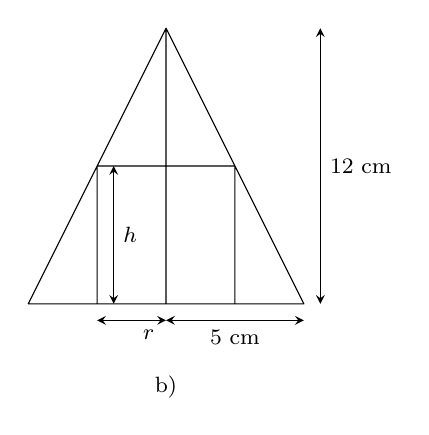
\begin{tikzpicture}[scale=0.7, font=\footnotesize, line join=round, line cap=round, >=stealth]
            \def \r{1.25} %bán kính đáy
            \def \h{2.5}
            \draw (0,2*\h)--(-2*\r,0)--(2*\r,0)--(0,2*\h)--(0,0) (-\r,0)--(-\r,\h)--(\r,\h)--(\r,0);
            \draw[<->] (-\r+0.3,0)--(-\r+0.3,\h);
            \node at (-\r+0.3,\h/2) [right]{$h$};
            \draw[<->] (-\r,-0.3)--(0,-0.3);
            \node at (-\r/4,-0.3) [below]{$r$};
            \draw[<->] (0,-0.3)--(2*\r,-0.3);
            \node at (\r,-0.3) [below]{$5$ cm};
            \draw[<->] (2*\r+0.3,0)--(2*\r+0.3,2*\h);
            \node at (2*\r+0.3,\h) [right]{$12$ cm};
            \node at (0,-1.5){\text{b)}};
        \end{tikzpicture}
    \end{center}
    \choiceTF
    {\True công thức tính bán kính $r$ của đáy hình trụ theo chiều cao $h$ của nó là $r=\dfrac{5\cdot (12-h)}{12}$}
    {\True Biểu thức $V(h)=\dfrac{25\pi\cdot h\cdot (12-h)^2}{144}$ biểu thị thể tích khối trụ theo $h$}
    {khối trụ có thể tích lớn nhất khi $h=12$}
    {\True khối trụ có thể tích lớn nhất bằng $\dfrac{400\pi}{9}$}
    \loigiai{
        \begin{center}
            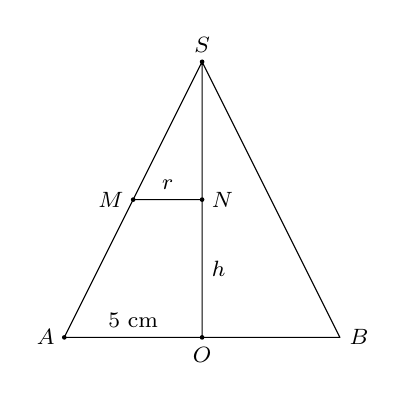
\begin{tikzpicture}[scale=0.7, font=\footnotesize, line join=round, line cap=round, >=stealth]
                \def \r{1.25} %bán kính đáy
                \def \h{2.5}
                \coordinate[label=above:$S$] (S) at (0,2*\h);
                \coordinate[label=left:$A$] (A) at (-2*\r,0);
                \coordinate[label=right:$B$] (B) at (2*\r,0);
                \coordinate[label=below:$O$] (O) at (0,0);
                \coordinate[label=left:$M$] (M) at (-\r,\h);
                \coordinate[label=right:$N$] (N) at (0,\h);
                \node at (-\r/2,\h) [above]{$r$};
                \node at (0,\h/2) [right]{$h$};
                \node at (-\r,0) [above]{$5$ cm};
                \draw (S)--(A)--(B)--(S)--(O) (M)--(N);
                \foreach \diem in {S,A,O,M,N}	\fill (\diem)circle(1.2pt);
            \end{tikzpicture}
        \end{center}
        \begin{itemchoice}
            \itemch {\bf Đúng}. Giả sử ta có hình vẽ như hình trên.\\
            Khi đó $\triangle SMN\backsim \triangle SAO$ nên
            $\dfrac{MN}{AO}=\dfrac{SN}{SO} \Leftrightarrow \dfrac{r}{5}=\dfrac{12-h}{12}$.\\
            Suy ra $r=\dfrac{5\cdot (12-h)}{12}$.
            \itemch {\bf Đúng}. Thể tích khối trụ là
            $V=h\pi\cdot r^2=h\pi\cdot\left(\dfrac{5\cdot (12-h)}{12}\right)^2=\dfrac{25\pi\cdot h\cdot (12-h)^2}{144}$.
            \itemch {\bf Sai}. Ta có $V(h)=\dfrac{25\pi\cdot h\cdot (12-h)^2}{144}=\dfrac{25\pi}{144}\cdot (h^3-24h^2+144h)$, với $h\in (0;12)$.\\
            $\Rightarrow V'(h)=\dfrac{25\pi}{144}\cdot (3h^2-48h+144)$; $V'(h)=0 \Leftrightarrow \hoac{& h=4\\& h=12.}$
            Bảng biến thiên
            \begin{center}
                
\begin{tikzpicture}
                    \tkzTabInit[nocadre=false,lgt=1.5,espcl=4,deltacl=0.6]
                    {$h$ /0.6,$V'(h)$ /0.6,$V(h)$ /2}
                    {$0$,$4$,$12$}
                    \tkzTabLine{,+,$0$,-,$0$}
                    \tkzTabVar{-/$0$, +/$\dfrac{400\pi}{9}$,-/$0$}
                \end{tikzpicture}
            \end{center}
            Vậy khi $h=4$ thì thể tích $V(h)$ lớn nhất.
            \itemch {\bf Đúng}.
        \end{itemchoice}
    }
\end{ex}
%2
\begin{ex}%[2D1V3-6]
    Hình bên dưới cho biết sự thay đổi của nhiệt độ ở một thành phố trong một ngày.
    \begin{center}
        \begin{tikzpicture}[ line join=round, line cap=round, >=stealth, transform shape, scale = 1,x=0.25cm,y=0.1cm,
            declare function={xmin=-2; xmax=28; ymin=-4; ymax=40; }
            ]
            \draw[->] (xmin,0)--(0,0) node[below left]{$O$}--(xmax,0) node[below right]{$x$ (giờ)};
            \draw[->] (0,ymin)--(0,ymax) node[left]{$t$ ($^\circ C$)};
            \foreach \x/\g in {4/-90,8/-90,12/-90,16/-90,20/-90,24/-90}
            \draw[thin] (\x,2pt)--(\x,-2pt) + (\g:3mm) node {$\x$};
            %Vẽ các điểm trên trục Oy
            \foreach \y/\g in {25/180}
            \draw[thin] (2pt,\y)--(-2pt,\y) + (\g:3mm) node {$\y$};
            \path
            (0,25) coordinate (25)
            (4,20) coordinate (20)
            (8,31) coordinate (31)
            (12,28) coordinate (28)
            (16,34) coordinate (34)
            (20,27) coordinate (27)
            (24,24) coordinate (24);
            \draw [dashed] (4,0)--(4,20) (8,0)--(8,31) (12,0)--(12,28) (16,0)--(16,34) (20,0)--(20,27) (24,0)--(24,24);
            \draw[smooth, thick, red]
            (25) .. controls +(-10:1) and +(-180:1) .. (20)
            (20) .. controls +(0:1) and +(-180:1) .. (31)
            (31) .. controls +(0:1) and +(160:1) .. (28)
            (28) .. controls +(0:1) and +(-180:2) .. (34)
            (34) .. controls +(0:1.5) and +(130:1.5) .. (27)
            (27) .. controls +(-60:1.5) and +(-180:2) .. (24);
            \foreach \x in {20,31,28,34,27,24}
            \fill (\x) +(90:3mm) node {$\x$};
        \end{tikzpicture}
    \end{center}
    \choiceTF
    {Nhiệt độ cao nhất trong ngày là $28^{\circ} \mathrm{C}$}
    {Nhiệt độ cao nhất trong ngày là $40^{\circ} \mathrm{C}$}
    {\True Nhiệt độ cao nhất trong ngày là $34^{\circ} \mathrm{C}$}
    {\True Nhiệt độ thấp nhất trong ngày là $20^\circ$C}
    \loigiai{
        \begin{itemchoice}
            \itemch {\bf Sai}. Nhiệt độ cao nhất trong ngày là $28^{\circ} \mathrm{C}$.
            \itemch {\bf Sai}. Nhiệt độ cao nhất trong ngày là $40^{\circ} \mathrm{C}$.
            \itemch {\bf Đúng}. Nhiệt độ cao nhất trong ngày là $34^{\circ} \mathrm{C}$.
            \itemch {\bf Đúng}. Nhiệt độ thấp nhất trong ngày là $20^\circ$C.
    \end{itemchoice}}
\end{ex}
%3
\begin{ex}%[2D1V3-6]
    Một công ty kinh doanh bất động sản có $20$ căn hộ cho thuê. Biết rằng nếu cho thuê mỗi căn hộ với giá $2$ triệu đồng/$1$ tháng thì tất cả các căn hộ đều có người thuê. Nhưng cứ mỗi lần tăng giá cho thuê mỗi căn hộ thêm $200$ nghìn đồng/$1$ tháng thì có thêm một căn hộ bỏ trống. Hỏi công ty nên cho thuê mỗi căn hộ giá bao nhiêu để tổng số tiền thu được là lớn nhất?
    \choiceTF
    {\True Cứ mỗi lần tăng giá cho thuê mỗi căn hộ thêm $200$ nghìn đồng/$1$ tháng thì có thêm một căn hộ bỏ trống.}
    {\True Gọi số lần tăng $200$ nghìn đồng/$1$ tháng mỗi căn hộ là $x$ $(x\in\mathbb{N}$ thì Số căn hộ có người thuê là $20-x$ $(0\le x \le 20)$}
    {Công ty cho thuê mỗi căn hộ giá $2{,}5$ triệu đồng thì tổng số tiền thu được là lớn nhất}
    {\True Công ty thu được số tiền lớn nhất bằng $45$ triệu đồng}
    \loigiai{
        Cứ mỗi lần tăng giá cho thuê mỗi căn hộ thêm $200$ nghìn đồng/$1$ tháng thì có thêm một căn hộ bỏ trống.\\
        Gọi số lần tăng $200$ nghìn đồng/$1$ tháng mỗi căn hộ là $x$ $(x\in\mathbb{N})$.\\
        Số căn hộ có người thuê là $20-x$ $(0\le x \le 20)$.\\
        Tổng số tiền thu được là $(2000+200x)(20-x)$.\\
        Xét hàm số $f(x)=(2000+200x)(20-x)=-200x^2+2000x+40000$ trên khoảng $(0;20)$.\\
        $f'(x)=-400x+2000$, $f'(x)=0\Leftrightarrow -400x+2000=0\Leftrightarrow x=5 $.\\
        Bảng biến thiên hàm số $f(x)$ trên khoảng $(0;20)$.
        \begin{center}
            
\begin{tikzpicture}
                \tkzTabInit[lgt=1.2,espcl=4.5,deltacl=0.8]
                {$x$/.8,$f'(x)$/.8,$f(x)$/2.5} {$0$,$5$,$20$}
                \tkzTabLine{,+,0,-,}
                \tkzTabVar{-/$40000$,+/$45000$,-/$0$}
            \end{tikzpicture}
        \end{center}
        Từ bảng biến thiên suy ra $\max\limits_{(0;20)} f(x)=f(5)=45000$ tại $x=5$.\\
        Vậy công ty nên cho thuê mỗi căn hộ giá $2000+200\cdot5=3000$ nghìn đồng (ba triệu đồng) thì tổng số tiền thu được là lớn nhất.
        \begin{itemchoice}
            \itemch {\bf Đúng}. Cứ mỗi lần tăng giá cho thuê mỗi căn hộ thêm $200$ nghìn đồng/$1$ tháng thì có thêm một căn hộ bỏ trống.
            \itemch {\bf Đúng}. Gọi số lần tăng $200$ nghìn đồng/$1$ tháng mỗi căn hộ là $x$ $(x\in\mathbb{N}$ thì Số căn hộ có người thuê là $20-x$ $(0\le x \le 20)$.
            \itemch {\bf Sai}. Công ty cho thuê mỗi căn hộ giá $3$ triệu đồng thì tổng số tiền thu được là lớn nhất
            \itemch {\bf Đúng}. Công ty thu được số tiền lớn nhất bằng $45$ triệu đồng.
        \end{itemchoice}
    }
\end{ex}
%4
\begin{ex}%[2D1V3-6]
    Có hai xã $A$, $B$ cùng ở một bên bờ sông Lam, khoảng cách từ hai xã đó đến bờ sông lần lượt là $AA'=500$ m, $BB'=600$ m và người ta đo được $A'B'=2\,200$ m {\it Hình 1}. Các kĩ sư muốn xây một trạm cung cấp nước sạch nằm bên bờ sông Lam cho dân hai xã. Để tiết kiệm chi phí, các kĩ sư cần phải chọn vị trí $M$ của trạm cung cấp nước sạch đó trên đoạn $A'B'$ sao cho tổng khoảng cách từ hai xã đến vị trí $M$ là nhỏ nhất.
    \begin{center}
        \begin{tikzpicture}
            \path
            (0:0) coordinate (A')
            (0:6) coordinate (B')
            (0:2) coordinate (M)
            ($(A')+(90:2.5)$) coordinate (A)
            ($(B')+(90:3)$) coordinate (B)
            ;
            \fill[cyan!50] (-1.5,-1) rectangle (7.5,0);
            \draw[thick] (A')--node[left]{$500 \text{(m)}$}(A)--(M)--(B)--node[right]{$600 \text{(m)}$}(B');
            \foreach \i/\j in{A'/-100,B'/-80,A/100,B/80,M/-90}{\fill [black](\i) circle (1pt) ($(\i)+(\j:3mm)$) node {$\i$};}
            \draw [dashed,<->]	(0,.6)--(6,.6) node[pos=0.75,sloped,above]{$2\,200\text{(m)}$}; %Tùy chọn sloped,above,below
            \node at (3,-1.5){\it Hình 37};
        \end{tikzpicture}
    \end{center}
    \choiceTF
    {\True Đặt $A'M=x$, $(0<x<2200)$, $B'M=2200-x$}
    {\True Ta có $AM=\sqrt{x^2+500^2}$, $BM=\sqrt{(2200-x)^2+600^2}$}
    {\True Giá trị nhỏ nhất của tổng khoảng cách từ hai xã đó đến bờ sông đạt được tại vị trí $M$ cách điểm $A'$ là $1000$ m}
    {\True Giá trị nhỏ nhất của tổng khoảng cách đó bằng $2460$ m}
    \loigiai{
        \begin{center}
            \begin{tikzpicture}
                \path
                (0:0) coordinate (A')
                (0:6) coordinate (B')
                (0:2) coordinate (M)
                ($(A')+(90:2.5)$) coordinate (A)
                ($(B')+(90:3)$) coordinate (B)
                ;
                \draw[thick] (A')--node[left]{$500 \text{(m)}$}(A)--(M)--(B)--node[right]{$600 \text{(m)}$}(B') (A')--(B');
                \foreach \i/\j in{A'/-100,B'/-80,A/100,B/80,M/-90}{\fill [black](\i) circle (1pt) ($(\i)+(\j:3mm)$) node {$\i$};}
                \draw [dashed,<->]	(0,.6)--(6,.6) node[pos=0.75,sloped,above]{$2\,200\text{(m)}$}; %Tùy chọn sloped,above,below
                \node at (3,-1.5){\it Hình 37};
            \end{tikzpicture}
        \end{center}
        Đặt $A'M=x$, $(0<x<2200)$, $B'M=2200-x$.\\
        Ta có $AM=\sqrt{x^2+500^2}$, $BM=\sqrt{(2200-x)^2+600^2}$.\\
        Khi đó tổng khoảng cách từ hai xã đến vị trí $M$ là $AM+BM= \sqrt{x^2+500^2}+\sqrt{(2200-x)^2+600^2} $.\\
        Xét hàm số $f(x)= \sqrt{x^2+500^2}+\sqrt{(2200-x)^2+600^2}$ trên khoảng $(0<x<2200)$.\\
        %$f(x)=\sqrt{x^2+500}+\sqrt{x^2-4400x+4840600}$ .\\
        $f^\prime (x)=\dfrac{x}{\sqrt{x^2+500^2}}-\dfrac{2200-x}{\sqrt{(2200-x)^2+600^2}}$, $f^\prime (x)=0\Leftrightarrow \dfrac{x}{\sqrt{x^2+500^2}}=\dfrac{2200-x}{\sqrt{(2200-x)^2+600^2}}$\\
        $\Leftrightarrow \dfrac{x^2}{x^2+500^2}=\dfrac{(2200-x)^2}{(2200-x)^2+600^2}$\\
        $\Leftrightarrow \dfrac{x^2+500^2}{x^2}=\dfrac{(2200-x)^2+600^2}{(2200-x)^2}$\\
        $\Leftrightarrow 1+\dfrac{500^2}{x^2}=1+\dfrac{600^2}{(2200-x)^2}$\\
        $\Leftrightarrow \dfrac{25}{x^2}=\dfrac{36}{(2200-x)^2}$\\
        $\Leftrightarrow \dfrac{5}{x}=\dfrac{6}{2200-x}\Leftrightarrow x=1000$, vì $ x>0$.\\
        Bảng biến thiên hàm số $f(x)$ trên khoảng $\left( 0;2200\right)$.
        \begin{center}
            
\begin{tikzpicture}
                \tkzTabInit[lgt=1.2,espcl=4.5,deltacl=0.6]
                {$x$/1,$f'(x)$/1,$f(x)$/3} {$0$,$1000$,$2200$}
                \tkzTabLine{,-,0,+,}
                \tkzTabVar{+/$2780$,-/$2460$,+/$2856$}
            \end{tikzpicture}
        \end{center}
        Vậy giá trị nhỏ nhất của tổng khoảng cách từ hai xã đó đến bờ sông là khoảng $2460$ m, tại vị trí $M$ cách điểm $A'$ là $1000$ m.
        \begin{itemchoice}
            \itemch {\bf Đúng}. Đặt $A'M=x$, $(0<x<2200)$, $B'M=2200-x$.
            \itemch {\bf Đúng}. Ta có $AM=\sqrt{x^2+500^2}$, $BM=\sqrt{(2200-x)^2+600^2}$.
            \itemch {\bf Đúng}. Giá trị nhỏ nhất của tổng khoảng cách từ hai xã đó đến bờ sông đạt được tại vị trí $M$ cách điểm $A'$ là $1000$ m.
            \itemch {\bf Đúng}. Giá trị nhỏ nhất của tổng khoảng cách đó bằng $2460$ m.
        \end{itemchoice}
    }
\end{ex}
%5
\begin{ex}%[2D1V3-6]
    Một trang sách có dạng hình chữ nhật với diện tích là $384$ cm$^2$. Sau khi để lề trên và lề dưới đều là $3$ cm, để lề trái và lề phải đều là $2$ cm. Phần còn lại của trang sách được in chữ.
    \choiceTF
    {\True Gọi $x$ cm là chiều dài lề trên và lề dưới.
        Chiều dài lề trái và lề phải là $\dfrac{384}{x}$ cm. Điều kiện $4<x<64$}
    {Diện tích phần in chữ trên trang sách là $S(x)=(x-4)\left(\dfrac{384}{x}-4\right)$}
    {\True Trang sách có diện tích lớn nhất bằng $216$ cm$^2$}
    {\True Kích thước tối ưu của trang sách lần lượt là $16$ cm và $24$ cm}
    \loigiai{
        \immini{
            Gọi $x$ cm là chiều dài lề trên và lề dưới.\\
            Chiều dài lề trái và lề phải là $\dfrac{384}{x}$ cm. Điều kiện $4<x<64$.\\
            Diện tích phần in chữ trên trang sách là $S(x)=(x-4)\left(\dfrac{384}{x}-6 \right)$.\\
            Xét hàm số $f(x)= (x-4)\left(\dfrac{384}{x}-6 \right) =\dfrac{-6x^2-408x-1536}{x}$ trên khoảng $(4;64)$.\\
            $f'(x)=\dfrac{-6x^2+1536}{x^2}$.\\
            $f'(x)=0\Leftrightarrow \dfrac{-6x^2+1536}{x^2}=0\Leftrightarrow\hoac{& x=-16 \notin (4;64)\\&x=16\in (4;64)}$
        }{
            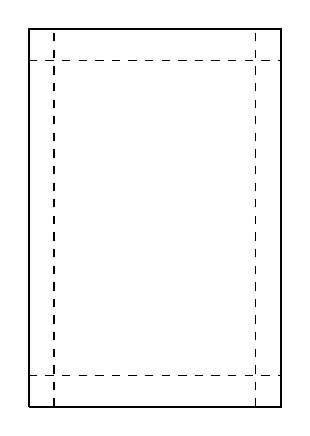
\begin{tikzpicture}[scale=.8]
                \def \a {4} \def \b {6}
                \draw[dashed,thin] (0,.5)--++(0:\a) (0,\b-.5)--++(0:\a) (.4,0)--++(90:\b) (\a-.4,0)--++(90:\b);
                \draw[thick] (0:0)--++(0:\a)--++(90:\b)--++(180:\a)--++(-90:\b);
            \end{tikzpicture}
        }
        \noindent
        Bảng biến thiên hàm số $f(x)$ trên khoảng $(6;96)$
        \begin{center}
            
\begin{tikzpicture}
                \tkzTabInit[lgt=1.2,espcl=2.5,deltacl=0.6]
                {$x$/0.6,$f'(x)$/0.6,$f(x)$/2} {$4$,$16$,$64$}
                \tkzTabLine{,+,0,-,}
                \tkzTabVar{-/$0$,+/$216$,-/$0$}
            \end{tikzpicture}
        \end{center}
        Từ bảng biến thiên suy ra $\max\limits_{(4;64)} f(x)=f(16)=216$.\\
        Do đó chiều dài lề trên và lề dưới của trang sách là $16$ cm, dài lề trái và lề phải của trang sách là $\dfrac{384}{16}=24$ cm thì phần in chữ trên trang sách có diện tích lớn nhất bằng $216$ cm$^2$.
        \begin{itemchoice}
            \itemch {\bf Đúng}. Gọi $x$ cm là chiều dài lề trên và lề dưới.
            Chiều dài lề trái và lề phải là $\dfrac{384}{x}$ cm. Điều kiện $4<x<64$.
            \itemch {\bf Sai}. Diện tích phần in chữ trên trang sách là $S(x)=(x-4)\left(\dfrac{384}{x}-4\right)$
            \itemch {\bf Đúng}. Trang sách có diện tích lớn nhất bằng $216$ cm$^2$
            \itemch {\bf Đúng}. Kích thước tối ưu của trang sách lần lượt là $16$ cm và $24$ cm.
        \end{itemchoice}
    }
\end{ex}
\BTTL
\begin{ex}%[TeX hóa SGK CTST 12]%[Nguyen Huynh]%[2D1H3-2]
    Tìm giá trị lớn nhất và giá trị nhỏ nhất của hàm số có đồ thị được cho ở hình sau
    \begin{center}
        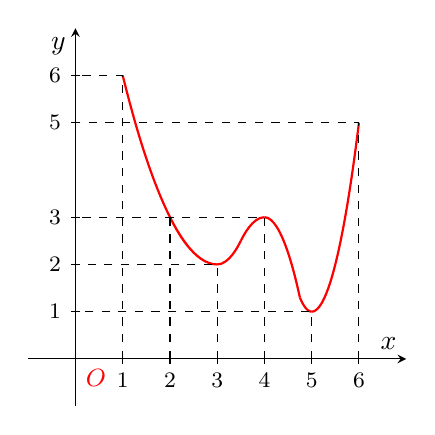
\begin{tikzpicture}[>=stealth,scale=0.6]
            %	\draw[line width=0.1pt,dashed] (0,0) grid (6,6);
            \draw[-> ] (-1,0) -- (7,0)node[above left] {$x$};
            \draw[-> ] (0,-1) -- (0,7)node[below left] {$y$};
            \draw [thick,red](0,0) node[below right] {\small $O$};
            \draw [thick,red](1,6) parabola bend (3,2) (2,3);
            \draw [thick,red](3,2) parabola (3.5,2.5);
            \draw [thick,red](3.5,2.5) parabola [bend at end] (4,3);
            \draw [thick,red](4,3) parabola (4.75,1.3);
            \draw [thick,red](4.75,1.3) parabola[bend at end] (5,1);
            \draw [thick,red](5,1) parabola (6,5);
            \foreach \x in {1,2,3,4,5,6}\draw (\x,0.1)--(\x,-0.1) node [below] {\footnotesize $\x$};
            \foreach \y in {5,6,1,2,3}\draw (0.1,\y)--(-0.1,\y) node [left] {\footnotesize $\y$};
            \draw[dashed] (1,0) -- (1,6) -- (0,6);
            \draw[dashed] (2,0) -- (2,3);
            \draw[dashed] (3,0) -- (3,2) -- (0,2);
            \draw[dashed] (4,0) -- (4,3) -- (0,3);
            \draw[dashed] (5,0) -- (5,1) -- (0,1);
            \draw[dashed] (6,0) -- (6,5) -- (0,5);
        \end{tikzpicture}
    \end{center}
    \shortans{$M=6$, $m=1$}
\end{ex}
\begin{ex}%[2D1V3-2]%[Dự án EX-TF-TLN-2024 - Đợt 1]%[Thành Đức Trung]
    Cho $(P)\colon y=x^2$ và $A\left(-2;\dfrac{1}{2}\right)$. Gọi $M$ là một điểm bất kì thuộc $(P)$. Tìm khoảng cách $MA$ nhỏ nhất (làm tròn đến chữ số thập phân thứ hai sau dấu phẩy).
    \shortans{$1{,}12$}
    \loigiai{
        Ta có: $M\in (P)\Rightarrow M\left(t;t^2\right), t\in \mathbb{R}$.
        \[
        MA=\sqrt{\left(t+2\right)^2+\left(t^2-\dfrac{1}{2}\right)^2}=\sqrt{t^4+4t+\dfrac{17}{4}}.
        \]
        Xét $f(t)=t^4+4t+\dfrac{17}{4}$ trên $\mathbb{R}$ có $f'(t)=4t^3+4$ nên $f'(t)=0\Leftrightarrow t=-1$.\\
        Bảng biến thiên:
        \begin{center}
            
\begin{tikzpicture}[>=stealth]
                \tkzTabInit[lgt=1.5,espcl=3]
                {$t$/.7,$f'(t)$/.7,$f(t)$/1.5}
                {$-\infty$,$-1$,$+\infty$}
                \tkzTabLine{,-,z,+,}
                \tkzTabVar{+/$+\infty$,-/$\dfrac{5}{4}$,+/$+\infty$}
            \end{tikzpicture}
        \end{center}
        Suy ra: $f(t)\geqslant \dfrac{5}{4}\Rightarrow AM\geqslant \dfrac{\sqrt{5}}{2}$.\\
        Vậy khoảng cách $MA$ bé nhất bằng $\dfrac{\sqrt{5}}{2} \approx 1{,}12$ khi $M\left(-1;1\right)$.
    }
\end{ex}
\begin{ex}%[2D1V3-6]
    \immini{
        Sự phân huỷ của rác thải hữu cơ có trong nước sẽ làm tiêu hao oxygen hoà tan trong nước. Nồng độ oxygen (mg/l) trong một hồ nước sau $t$ giờ $(t \geq 0)$ khi một lượng rác thải hữu cơ bị xả vào hồ được xấp xỉ bởi hàm số (có đồ thị như đường màu đỏ ở hình bên)
        $$
        y(t)=5-\frac{15 t}{9 t^2+1}.
        $$
        (Theo: https://www.researchgate.net/publication/264903978$\_$Microrespirometric$\_$ characterization$\_$\\of$\_$activated$\_$sludge$\_$inhibition$\_$by$\_$copper$\_$and$\_$zinc)\\
        Vào các thời điểm nào nồng độ oxygen trong nước cao nhất?
    }{
        \begin{tikzpicture}[>=stealth,x=1cm,y=0.3cm,scale=2,font=\footnotesize]
            \draw[->] (-0.5,0) -- (4,0) node[below] {$t$};
            \draw[->] (0,-1) -- (0,6) node[left] {$y$};
            \filldraw (0,0) circle (1pt)node[below left]{$O$};
            \draw[domain=0:4,samples=200,red] plot (\x,{5-(15*(\x))/(9*(\x)^2+1)});
            \draw[dashed] (0,5) node [left] {$5$}--(4,5);
            \foreach \x/\g in {1/-90,2/-90,3/-90}
            \draw[thin] (\x,2pt)--(\x,-2pt) + (\g:3mm) node {$\x$};
        \end{tikzpicture}
    }
    \shortans{$0$}
    \loigiai{
        Xét hàm số $y(t)=5-\dfrac{15t}{9t^2+1}$ xác định và liên tục trên khoảng $[0;+\infty)$ .\\
        Ta có $y'(t)=\dfrac{135t^2-15}{(9t^2+1)^2}=0\Leftrightarrow t=\dfrac{1}{3}$ (giờ).\\
        Mặt khác $\lim\limits_{t\to+\infty}y(t)=\lim\limits_{t\to+\infty}\left[5-\dfrac{15t}{9t^2+1}\right]=5$ và $\lim\limits_{t\to 0}y(t)=\lim\limits_{t\to 0}\left[5-\dfrac{15t}{9t^2+1}\right]=5$.\\
        Bảng biến thiên
        \begin{center}
            
\begin{tikzpicture}
                \tkzTabInit[espcl=3,lgt=1.5]
                {$t$/0.7,$y'(t)$/0.7,$y(t)$/2.1}
                {$0$,$\frac{1}{3}$,$+\infty$}
                \tkzTabLine{,-,0,+,}
                \tkzTabVar{+/$5$,-/$0$,+/$5$}
            \end{tikzpicture}
        \end{center}
        Từ bảng biến thiên, ta thấy $\min\limits_{[0;+\infty)}y(x)=0$ và $\mathop{\rm{max}}\limits_{[0;+\infty)}y(x)=5$.
    }
\end{ex}
%2
\begin{ex}%[2D1V3-6]
    Từ một tấm bìa hình chữ nhật có chiều rộng $30 \mathrm{~cm}$ và chiều dài $80 \mathrm{~cm}$ (Hình $a$), người ta cắt ở bốn góc bốn hình vuông có cạnh $x(\mathrm{~cm})$ với $5 \leq x \leq 10$ và gấp lại để tạo thành chiếc hộp có dạng hình hộp chữ nhật không nắp như (Hình $b$). Tìm $x$ để thể tích chiếc hộp là lớn nhất (kết quả làm tròn đến hàng phần trăm).
    \shortans{$6{,}67$}
    \begin{multicols}{2}
        \begin{center}
            \begin{tikzpicture}[line join=round, line cap=round,thick]
                \coordinate (A) at (0,3);
                \coordinate (B) at (5,3);
                \coordinate (D) at (0,0);
                \coordinate (C) at ($(B)+(D)-(A)$);
                \draw(A)--(B)--(C)--(D)--cycle;
                \draw (0,0) rectangle (1,1) (A) rectangle (1,2) (B) rectangle (4,2) (4,1) rectangle (C);
                \draw[dashed] (1,1) rectangle (4,2);
                %	\foreach \i/\g in {A/90,B/90,C/-90,D/-90}{\draw[fill=black](\i) circle (1pt) ($(\i)+(\g:3mm)$) node[scale=1]{$\i$};}
                \draw (0,.5) node [left] {$x$};
                \draw (.5,0) node [below] {$x$};
                \draw (0,2.5) node [left] {$x$};
                \draw (0.5,3) node [above] {$x$};
                %%%%%%%%%
                \draw (4.5,0) node [below] {$x$};
                \draw (5,0.5) node [right] {$x$};
                \draw (5,2.5) node [right] {$x$};
                \draw (4.5,3) node [above] {$x$};
                %%%%%%%%
                \draw[<->] (-1,0)--(-1,3);
                \draw[<->] (0,-1)--(5,-1);
                \draw (-1.2,.8) node[left,rotate=-90] {$30$cm};
                \draw (3.2,-0.8) node[left,rotate=0] {$80$cm};
            \end{tikzpicture}
            \begin{center}
                a)
            \end{center}
        \end{center}
        %%%%%%%%%%%%%%
        \begin{center}
            \begin{tikzpicture}[line join=round, line cap=round,thick,scale=.8]
                \def\a{3.5}
                \path 	(0:0) coordinate (A)
                ++(0:\a) coordinate (D)
                ++(-130:\a/2) coordinate (C)
                ($(A)+(C)-(D)$) coordinate (B)
                ($(A)+(90:\a)$) coordinate (A')
                ($(B)+(90:\a)$) coordinate (B')
                ($(C)+(90:\a)$) coordinate (C')
                ($(D)+(90:\a)$) coordinate (D');
                \draw[dashed,thick] 	(B)--(A)--(D)	(A)--(A');
                \draw[thick] 	(C)--(C') 	(D)--(D') 	(B)--(B') 	(B)--(C)--(D) (A')--(B')--(C')--(D')--cycle;
                %\foreach \x/\g in {A/180,B/180,C/0,D/0,A'/180,B'/180,C'/0,D'/0}\fill[black] 	(\x) circle (1pt)	($(\g:4mm)+(\x)$) node {$\x$};
            \end{tikzpicture}
        \end{center}
        \begin{center}
            b)
        \end{center}
    \end{multicols}
    \loigiai{
        Thể tích chiếc hộp là $V(x)=x(30-2 x)(80-2 x)=2400 x-220 x^2+4 x^3$ với $5 \leq x \leq 10$.\\
        Ta có $V'(x)=12 x^2-440 x+2400$;
        $V'(x)=0 \Leftrightarrow x=\dfrac{20}{3}$ hoặc $x=30$ (loại vì không thuộc $[5;10]$).
        \begin{center}
            $V(5)=7000$; $V\left(\dfrac{20}{3}\right)=\dfrac{200000}{27}$; $V(10)=6000$.
        \end{center}
        Do đó $\max \limits_{[5 ; 10]} V(x)=\dfrac{200000}{27}$ khi $x=\dfrac{20}{3}$.
        Vậy để thể tích chiếc hộp là lớn nhất thì $x=\dfrac{20}{3} \mathrm{~cm}$.}
\end{ex}
%3
\begin{ex}%[TeX hóa SGK CTST 12]%[Nguyen Huynh]%[2D1H3-6]
    Khi làm nhà kho, bác An muốn cửa sổ có dạng hình chữ nhật với chu vi bằng $4 \mathrm{~m}$ . Tìm kích thước khung cửa sổ sao cho diện tích cửa sổ lớn nhất (để hứng được nhiều ánh sáng nhất)?
    \shortans{$1$}
    \loigiai{
        Gọi chiều dài của khung cửa sổ là $x$ (mét). Điều kiện $0<x<2$.\\
        Suy ra chiều rộng của khung cửa sổ là $2-x$ (mét).\\
        Khi đó diện tích của khung cửa sổ là $x\left(2-x\right)=-x^2+2x$.\\
        Đặt $f(x)=-x^2+2x\Rightarrow f'(x)=-2x+2=0\Leftrightarrow x=1$. Ta có bảng biến thiên như sau
        \begin{center}
            
\begin{tikzpicture}[font=\normalsize,t style/.style={style=solid}]
                %dòng khai báo
                \tkzTabInit[lgt=1.2,espcl=2.5,deltacl=0.5]
                {$x$ /0.75, $f'(x)$/0.75, $f(x)$/2}
                {$ 0$,$ 1 $,$ 2$}
                %dòng xét dấu
                \tkzTabLine{ , +,0 , -, } % z, t, d;
                %dòng biến thiên
                \tkzTabVar{-/$0$,+/$1$,-/$0$} %+ hoac-
            \end{tikzpicture}
        \end{center}
        Như bảng biến thiên ta thấy được diện tích khung của sổ lớn nhất khi $x=1$ hay khung cửa có dạng hình vuông cạnh $1$ mét.}
\end{ex}
%4
\begin{ex}%[2D1V3-6]
    Hộp sữa $1$ lít được thiết kế dạng hình hộp chữ nhật với đáy là hình vuông cạnh $x$ cm. Tìm $x$ để diện tích toàn phần của hộp nhỏ nhất.
    \shortans{$10$}
    \loigiai{
        Thể tích hộp sữa là $1\ell=1\ \mathrm{dm}^3=1000\ \mathrm{cm}^3$ khi đó chiều cao của hộp sữa là $\dfrac{1000}{x^2}$ (cm).\\
        Đặt diện tích toàn phần của hộp sữa là $y=2x^2+4x\cdot \dfrac{1000}{x^2}=\dfrac{2x^3+4000}{x}$ (cm)$^2$.\\
        Xét $y'=\dfrac{4x^3-4000}{x^2}=0\Leftrightarrow x=10$ (cm).\\
        Ta có bảng biến thiên như sau
        \begin{center}
            
\begin{tikzpicture}[font=\normalsize,t style/.style={style=solid}]
                %dòng khai báo
                \tkzTabInit[lgt=1,espcl=2.65,deltacl=0.6]
                {$x$ /0.75, $y'$/0.75, $y$/2}
                {$ 0$,$ 10 $,$ +\infty$}
                %dòng xét dấu
                \tkzTabLine{ , -,0 , +, } % z, t, d;
                %dòng biến thiên
                \tkzTabVar{+/$+\infty$,-/$600$,+/$+\infty$} %+ hoac-
            \end{tikzpicture}
        \end{center}
        Vậy theo bảng biến thiên ta thấy $x=10$ (cm) thì diện tích toàn phần của hộp sữa sẽ nhỏ nhất là $600\ {\rm cm^2}$. }
\end{ex}
%5
\begin{ex}%[2D1V3-6]
    Trong một nhà hàng, mỗi tuần để chế biến $x$ phần ăn ($x$ lấy giá trị trong khoảng từ $30$ đến $120$) thì chi phí trung bình (đơn vị: nghìn đồng) của một phần ăn được cho bởi công thức
    $$C(x)=2x-230+\dfrac{7\,200}{x}.$$
    Tìm số phần ăn sao cho chi phí trung bình của một phần ăn là thấp nhất.
    \shortans{$4$}
    \loigiai{
        \begin{itemize}
            \item Tập xác định $\mathscr{D}=\mathbb{R}\setminus \{0\}$.
            \item Sự biến thiên\\
            Đạo hàm $y'=2-\dfrac{7\,200}{x^2}=\dfrac{2x^2-7\,200}{x^2}$; $y'=0 \Leftrightarrow \hoac{& x=-60 \text{ (loại)}\\& x=60 \text{ (nhận)}.}$\\
            Trên khoảng $(30;60)$, $y'<0$ nên hàm số nghịch biến trên khoảng đó.\\
            Trên khoảng $(60;120)$, $y'>0$ nên hàm số đồng biến trên khoảng đó.\\
            Hàm số đạt cực tiểu tại $x=60$, $y_{\text{CT}}=10$.\\
            Ta có $\lim\limits_{x\to -\infty} y=-\infty$; $\lim\limits_{x\to +\infty} y=+\infty$.\\
            Mà $\lim\limits_{x\to -\infty} \left[y-(2x-230)\right]=\lim\limits_{x\to -\infty} \dfrac{7\,200}{x}=0$; $\lim\limits_{x\to +\infty} \left[y-(2x-230)\right]=\lim\limits_{x\to +\infty} \dfrac{7\,200}{x}=0$.\\
            $\Rightarrow$ Đường thẳng $y=2x-230$ là tiệm cận xiên của đồ thị hàm số.\\
            Mặt khác $\lim\limits_{x\to 0^{-}} \left(2x-230+\dfrac{7\,200}{x}\right)=-\infty$; $\lim\limits_{x\to 0^{+}} \left(2x-230+\dfrac{7\,200}{x}\right)=+\infty$.\\
            $\Rightarrow$ Đường thẳng $x=0$ là tiệm cận đứng của đồ thị hàm số.\\
            Bảng biến thiên
            \begin{center}
                
\begin{tikzpicture}
                    \tkzTabInit[nocadre=true,lgt=1.2,espcl=4,deltacl=0.6]
                    {$x$ /0.6,$y'$ /0.6,$y$ /2}
                    {$30$,$60$,$120$}
                    \tkzTabLine{,-,$0$,+,}
                    \tkzTabVar{+/$70$,-/$10$,+/$70$}
                \end{tikzpicture}
            \end{center}
            \item Đồ thị
            \immini{
                Trên đoạn $[30;120]$, đồ thị của hàm số đã cho được biểu diễn như hình bên.
            }{
                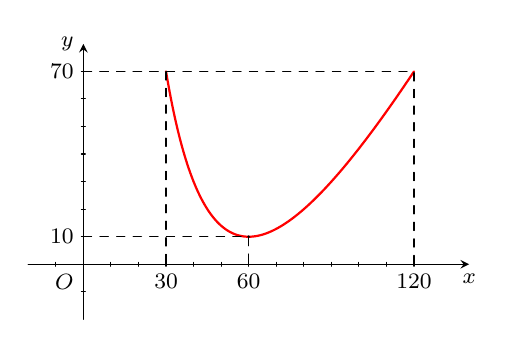
\begin{tikzpicture}[scale=0.7, font=\footnotesize, line join=round, line cap=round, >=stealth, xscale=0.5, yscale=0.5]
                    \def\a{2} \def\b{-23} \def\c{72} \def\m{1} \def\n{0} % Hệ số
                    \def\xt{-2} \def\xp{14} \def\yt{8} \def\yd{-2} % x_trái, x_phải, y_trên, y_dưới (giới hạn)
                    \draw[->] (\xt,0)--(\xp,0) node [below]{$x$};
                    \draw[->] (0,\yd)--(0,\yt) node [left]{$y$};
                    \node at (0,0) [below left]{$O$};
                    \clip (\xt+0.1,\yd+0.1) rectangle (\xp-0.1,\yt-0.1);
                    \draw[thick,red,smooth,samples=300,domain=3:12,red] plot(\x,{(\a*(\x)^2+\b*(\x)+\c)/(\m*(\x)+\n)});
                    \foreach \x in {-1,0,...,12}
                    \draw[shift={(\x,0)},color=black] (0pt,2pt) -- (0pt,-2pt);
                    \foreach \y in {-1,...,7}
                    \draw[shift={(0,\y)},color=black] (2pt,0pt) -- (-2pt,0pt);
                    \draw[dashed] (0,1)node [left]{$10$} -- (6,1) -- (6,0) node [below]{$60$};
                    \fill (6,1) circle (1.5pt);
                    \draw[dashed] (0,7)node [left]{$70$} -- (3,7) -- (3,0) node [below]{$30$};
                    \draw[dashed] (0,7) -- (12,7) -- (12,0) node [below]{$120$};
                \end{tikzpicture}
            }
        \end{itemize}
        Từ kết quả trên, để chi phí trung bình của một phần ăn là thấp nhất thì số phần ăn $x=60$.	}
\end{ex}
\Closesolutionfile{ans}